\documentclass[12pt,a4paper]{article}
\usepackage[utf8]{inputenc}
\usepackage[T1]{fontenc}
\usepackage[spanish]{babel}
\addto\captionsspanish{\renewcommand{\tablename}{Tabla}}
\AtBeginDocument{\ifdefined\decimalpoint\decimalpoint\fi} % punto decimal, como en el Punto 2
\usepackage{amsmath, amssymb, amsfonts}
\usepackage{geometry}
\usepackage{graphicx}
\usepackage{xcolor}
\usepackage{enumitem}
\usepackage{float}
\usepackage{booktabs}
\usepackage{array}
\usepackage[hidelinks]{hyperref}

\geometry{left=2.5cm, right=2.5cm, top=2.5cm, bottom=2.5cm}
\graphicspath{{imagenes/}}
\emergencystretch=3em

\newcommand{\dd}{\mathrm{d}}
\newcommand{\ee}{\mathrm{e}}
\newcommand{\media}[1]{\langle #1\rangle}

\title{\textbf{Oscilador de Mathieu-Duffing con ruido aditivo}}
\author{Jesús David Vitola González\\ Nicolas Lopez Prieto \\ [2pt] Física Computacional 2 -- Primer Examen Parcial, Punto 3}
\date{\today}

\begin{document}

\maketitle

\section{Fenomenología}

El oscilador de Mathieu-Duffing combina dos mecanismos no lineales. El primero es una rigidez que se modula periódicamente en el tiempo, $\omega_0^2+h\cos(\Omega t)$ cuando la frecuencia de modulación es cercana al doble de la frecuencia natural y la amplitud $h$ supera un umbral que depende del amortiguamiento, la posición de equilibrio se vuelve inestable y el oscilador crece de forma exponencial \cite{landau1976,nayfeh1979}. El segundo es una rigidez cúbica, $\beta x^{3}$, que con $\beta>0$ endurece el resorte y frena ese crecimiento, de modo que la amplitud se estabiliza en un valor finito.

A ese sistema se le añade ruido blanco aditivo de intensidad $\sigma$, que representa fluctuaciones del entorno. Una trayectoria individual no caracteriza al sistema: dos corridas con las mismas condiciones iniciales dan resultados distintos. Lo que tiene sentido estudiar son ensambles de realizaciones: medias, varianzas y distribuciones de probabilidad.

Las preguntas físicas y numéricas que se abordan son:
\begin{enumerate}[label=\textbf{\arabic*.}]
    \item ¿Qué esquema de integración estocástica (Euler-Maruyama o Heun) es más adecuado para este modelo, y por qué?
    \item ¿Cómo evolucionan la media, la varianza y la distribución de la posición en un ensamble de realizaciones?
    \item ¿Cómo depende la respuesta de la intensidad del ruido $\sigma$, por debajo y por encima del umbral de resonancia paramétrica?
    \item ¿Cómo se distinguen las fluctuaciones inducidas por el ruido de la dinámica determinista del sistema?
    \item ¿Qué revelan la autocorrelación y el espectro de potencia sobre la respuesta del sistema?
\end{enumerate}

\section{Modelo matemático, variables y parámetros}

\subsection{Ecuación de movimiento}

Sea $x$ la posición y $v=\dot x$ la velocidad. La ecuación que implementa el programa es
\begin{equation}
    \ddot x + \delta\,\dot x + \big[\omega_0^{2}+h\cos(\Omega t)\big]\,x + \beta\,x^{3} = \sigma\,\xi(t),
    \label{eq:mov}
\end{equation}
donde $\delta$ es el coeficiente de amortiguamiento, $\omega_0$ la frecuencia natural, $h$ y $\Omega$ la amplitud y la frecuencia de la modulación paramétrica, $\beta$ el coeficiente de la rigidez cúbica y $\sigma$ la intensidad del ruido. El proceso $\xi(t)$ es ruido blanco gaussiano, con $\media{\xi(t)}=0$ y $\media{\xi(t)\xi(t')}=\delta_{\mathrm{D}}(t-t')$ (delta de Dirac).

Como el ruido blanco no es una función en sentido ordinario, la ecuación se escribe como ecuación diferencial estocástica de primer orden en $(x,v)$, en la interpretación de Itô:
\begin{equation}
    \dd x = v\,\dd t, \qquad
    \dd v = a(t,x,v)\,\dd t + \sigma\,\dd W_t,
    \label{eq:sde}
\end{equation}
con
\begin{equation}
    a(t,x,v) = -\delta\,v - \big[\omega_0^{2}+h\cos(\Omega t)\big]\,x - \beta\,x^{3},
\end{equation}
y $W_t$ un proceso de Wiener. En una discretización con paso $\Delta t$, el incremento es $\Delta W_n=\sqrt{\Delta t}\,\eta_n$ con $\eta_n\sim\mathcal N(0,1)$ \cite{higham2001}.

\subsection{Propiedades}

\paragraph{Simetría.} La ecuación~\eqref{eq:mov} es impar en $x$: si $x(t)$ es solución (con el mismo ruido, reemplazado por $-\xi$), también lo es $-x(t)$. Por eso, en un ensamble que parte de una condición inicial simétrica, se espera $\media{x}=0$ a tiempos largos.

\paragraph{Resonancia paramétrica.} Para la parte lineal sin ruido ($\beta=0$, $\sigma=0$) y modulación con $\Omega\approx2\omega_0$, el análisis a primer orden en $h$ y $\delta$ da un umbral de inestabilidad
\begin{equation}
    h_c \approx 2\,\delta\,\omega_0,
    \label{eq:umbral}
\end{equation}
consistente con el tratamiento de Landau y Lifshitz \cite{landau1976}. Con $\delta=0.1$ y $\omega_0=1$, $h_c\approx0.2$. En los experimentos se usan $h=0.1$ (por debajo) y $h=0.5$ (por encima). Con $\beta>0$ el crecimiento se satura y aparece una respuesta subarmónica de frecuencia $\Omega/2$, es decir, de período $2T$ con $T=2\pi/\Omega$. Como la ecuación es impar, una solución de ese tipo cumple $x(t+T)=-x(t)$: las soluciones $x(t)$ y $-x(t)$ son la misma órbita desfasada un período del forzamiento.

\paragraph{Límite lineal con ruido.} Con $h=0$ y $\beta=0$ el modelo es un oscilador armónico amortiguado excitado por ruido blanco, con solución estacionaria gaussiana conocida \cite{gardiner2009}:
\begin{equation}
    \mathrm{Var}[x]=\frac{\sigma^{2}}{2\,\delta\,\omega_0^{2}},\qquad
    \mathrm{Var}[v]=\frac{\sigma^{2}}{2\,\delta}.
    \label{eq:ou}
\end{equation}
Este resultado exacto se usa para validar el código.

\subsection{Magnitudes estadísticas}

Con $N$ realizaciones $x^{(r)}(t)$, se estiman la media $\media{x}(t)=\frac1N\sum_r x^{(r)}$, la varianza muestral $\mathrm{Var}[x](t)=\frac{1}{N-1}\sum_r\big(x^{(r)}-\media{x}\big)^{2}$ y la densidad $P(x,t)$ mediante un histograma normalizado de las $x^{(r)}(t)$. Además:

\paragraph{Error fuerte.} Si $x_{\Delta t}(T)$ es la solución numérica con paso $\Delta t$ y $x_{\mathrm{ref}}(T)$ la de referencia, ambas calculadas con \emph{el mismo camino browniano}, el error fuerte es $\varepsilon(\Delta t)=\media{|x_{\Delta t}(T)-x_{\mathrm{ref}}(T)|}$, promediado sobre caminos. Si $\varepsilon\propto\Delta t^{p}$, $p$ es el orden fuerte.

\paragraph{Mapa estroboscópico.} Se registra $(x,v)$ en $t=nT$, con $T=2\pi/\Omega$. Una respuesta de período $T$ da un punto; de período $2T$, dos puntos; el ruido ensancha cada punto en una nube.

\paragraph{Autocorrelación y espectro.} Sobre la parte estacionaria, con la media restada, $C(\tau)=\media{x(t)\,x(t+\tau)}$, normalizada por $C(0)$. El espectro de potencia $S(\omega)$ se estima con el periodograma de $M$ muestras separadas $\Delta t_s$, $S(\omega)=\frac{\Delta t_s}{2\pi M}\big|\sum_{m}x_m\ee^{-\mathrm{i}\omega m\Delta t_s}\big|^{2}$, promediado sobre realizaciones (relación de Wiener-Khinchin \cite{gardiner2009}).

\subsection{Parámetros utilizados}

La Tabla~\ref{tab:param} resume los parámetros de cada conjunto de corridas. Todos los casos con modulación usan $\omega_0=1$, $\Omega=2=2\omega_0$ y $\beta=1$; en todos se integra con $\Delta t$ constante y $t=i\,\Delta t$.

\begin{table}[H]
\centering
\footnotesize
\setlength{\tabcolsep}{3pt}
\begin{tabular}{@{}p{3.1cm}p{5.2cm}p{6.6cm}@{}}
\toprule
Corrida & Modelo & Numéricos\\
\midrule
Simulación principal & $\delta=0.1$, $h=0.5$, $\sigma=0.2$; $x_0=0.5$, $v_0=0$ & Heun, $\Delta t=0.01$, $t_{\max}=200$, $N=200$, semilla $12345$\\
Validación lineal (3a) & $\delta=0.5$, $h=0$, $\beta=0$, $\sigma=0.5$; $x_0=v_0=0$ & $\Delta t\in\{0.2,0.1,0.05,0.025\}$, $t_{\max}=30$, $N=20\,000$\\
Convergencia fuerte (3b) & $\delta=0.1$, $h=0.5$, $\sigma=0.2$; $x_0=0.1$ & $T=5$, referencia con Heun y $\Delta t_f=T/8192$; $\Delta t\in\{4,8,16,32,64\}\Delta t_f$; $300$ caminos\\
Barrido en $\sigma$ (3c) & $\delta=0.1$, $h\in\{0.1,0.5\}$, $\sigma\in[0,0.3]$; $x_0=0.1$ & Heun, $\Delta t=0.01$, $t_{\max}=200$, ventana $t>100$, $N=300$\\
Estroboscópico (3d) & $\delta=0.1$, $h=0.5$, $\sigma\in\{0,0.05,0.2\}$; $x_0=0.1$ & $\Delta t=T/200$, $200$ períodos de transitorio y $1500$ de muestreo\\
Autocorrelación y espectro (3e) & $\delta=0.1$; ($h=0.1$, $\sigma=0.1$) y ($h=0.5$, $\sigma=0.05$); $x_0=0.1$ & Heun, $\Delta t=0.01$, transitorio $100$, $M=4096$ muestras cada $\Delta t_s=0.1$, $20$ realizaciones\\
\bottomrule
\end{tabular}
\caption{Parámetros de las corridas. Semillas fijas en el código de los experimentos: $1000+i$ y $2000+i$ (3a), $2024$ (3b), $10+i$ y $20+i$ (3c, para $h=0.1$ y $0.5$), $101$--$105$ (3c, estabilidad), $7$ (3d) y $31$ (3e).}
\label{tab:param}
\end{table}

\section{Método computacional y justificación}

\subsection{Generación del ruido}

Los incrementos de Wiener se generan con el motor \texttt{std::mt19937\_64} (Mersenne Twister de 64 bits \cite{matsumoto1998}) y la distribución \texttt{std::normal\_distribution}, como $\Delta W=\sqrt{\Delta t}\,\eta$ con $\eta\sim\mathcal N(0,1)$. El motor se inicializa con una semilla entera explícita. Hay un solo flujo para todo el ensamble: cada realización consume los números siguientes a los de la anterior, así que las realizaciones son distintas entre sí, pero la corrida completa se reproduce exactamente con la misma semilla, $N$, $\Delta t$ y $t_{\max}$. La semilla se registra en \texttt{parametros.txt}.

\subsection{Esquemas de integración}

Sea $a_n=a(t_n,x_n,v_n)$.

\begin{itemize}
    \item \textbf{Euler-Maruyama:} $x_{n+1}=x_n+\Delta t\,v_n$, $\;v_{n+1}=v_n+a_n\Delta t+\sigma\,\Delta W_n$. Con ruido aditivo su orden fuerte es 1 \cite{kloeden1992}.
    \item \textbf{Heun estocástico} (predictor-corrector, con el mismo $\Delta W_n$ en ambas etapas):
    \begin{align}
        \tilde x &= x_n+\Delta t\,v_n, &
        \tilde v &= v_n+a_n\Delta t+\sigma\,\Delta W_n,\\
        x_{n+1} &= x_n+\tfrac{\Delta t}{2}\,(v_n+\tilde v), &
        v_{n+1} &= v_n+\tfrac{\Delta t}{2}\,\big[a_n+a(t_{n+1},\tilde x,\tilde v)\big]+\sigma\,\Delta W_n.
    \end{align}
    \item \textbf{RK4 determinista} (solo con $\sigma=0$): control para comparar con la dinámica sin ruido.
\end{itemize}

\begin{table}[H]
\centering
\begin{tabular}{@{}lcc@{}}
\toprule
Método & Evaluaciones de $a$ por paso & Orden fuerte observado\\
\midrule
Euler-Maruyama & 1 & $\approx1.0$ ($1.00$--$1.03$)\\
Heun estocástico & 2 & $\approx1$ ($0.9$--$1.2$)\\
RK4 (control, $\sigma=0$) & 4 & --\\
\bottomrule
\end{tabular}
\caption{Esquemas implementados. Los órdenes provienen del experimento 3b.}
\end{table}

\subsection{Justificación}

\begin{itemize}
    \item El ruido es \emph{aditivo}: $\sigma$ no depende de $(x,v)$. Por eso las interpretaciones de Itô y de Stratonovich coinciden y el esquema de Heun, que converge a la solución de Stratonovich, es válido para este modelo.
    \item \textbf{Milstein no se implementó.} Su corrección sobre Euler-Maruyama es proporcional a la derivada del coeficiente de difusión respecto de la variable de estado; como aquí ese coeficiente es constante, la derivada es cero y Milstein coincide con Euler-Maruyama \cite{kloeden1992}. Habría sido un esquema redundante. Con ruido multiplicativo el caso sería distinto.
    \item Se eligió Heun para las corridas de física porque su sesgo en la varianza estacionaria es mucho menor (Tabla~\ref{tab:lineal}) y su error fuerte a igual $\Delta t$ es unas 6--7 veces menor (Tabla~\ref{tab:fuerte}), a un costo de dos evaluaciones de la fuerza por paso en lugar de una.
    \item El tiempo se calcula como $t=i\,\Delta t$ y no acumulando $t\mathrel{+}=\Delta t$, para no arrastrar error de redondeo dentro de $\cos(\Omega t)$.
    \item En el mapa estroboscópico se toma $\Delta t=T/200$, de modo que cada período contiene un número entero de pasos y el muestreo cae exactamente en $t=nT$.
    \item El programa verifica $\Delta t>0$, $t_{\max}>0$, $\delta>0$, $\omega_0>0$, $\Omega>0$, $\beta\ge0$, $\sigma\ge0$ y $N\ge1$, y detiene la corrida si $|x|>10^{6}$ (por ejemplo, con $\beta=0$ y $h$ por encima del umbral~\eqref{eq:umbral}, donde $x$ crece sin límite).
\end{itemize}

\section{Arquitectura del programa}

El código está escrito en C++ orientado a objetos con dos clases. La clase \texttt{Osc\_Mathieu\_Duffing} guarda el estado $(x,v)$ y contiene los integradores; la clase \texttt{Generador\_Ruido} encapsula el generador pseudoaleatorio.

\begin{itemize}
    \item \texttt{Osc\_Mathieu\_Duffing}: \texttt{Inicie(x0, v0)}; \texttt{calcularAceleracion(t, x, v, ...)}, que evalúa la parte determinista $a(t,x,v)$; \texttt{MuevaseEulerMaruyama}, \texttt{MuevaseHeun} y \texttt{MuevaseRK4}; y los accesores \texttt{Getx} y \texttt{Getv}.
    \item \texttt{Generador\_Ruido}: \texttt{Inicie(semilla)}, \texttt{calcularIncrementoWiener(dt)} y \texttt{GetSemilla()}.
\end{itemize}

El ruido \emph{no} vive dentro del oscilador: el incremento $\Delta W$ llega como argumento de \texttt{MuevaseEulerMaruyama} y \texttt{MuevaseHeun}. Así, dos esquemas pueden recibir exactamente el mismo ruido (como en el experimento 3b) y el oscilador puede probarse sin ruido.

\begin{table}[H]
\centering
\small
\begin{tabular}{@{}lp{10.5cm}@{}}
\toprule
Archivo & Función\\
\midrule
\texttt{Ruido.h / Ruido.cpp} & Clase \texttt{Generador\_Ruido}.\\
\texttt{MathieuDuffing.h / .cpp} & Clase \texttt{Osc\_Mathieu\_Duffing} y sus tres integradores.\\
\texttt{punto3.cpp} & Función \texttt{ejecutarPunto3()}: pide y valida los datos, corre el ensamble acumulando sumas de $x$, $x^2$, $v$ y $v^2$ en cada instante, y escribe \texttt{momentos.dat}, \texttt{trayectorias.dat} (cinco realizaciones), \texttt{x\_final.dat} y \texttt{parametros.txt}. Genera los scripts de gnuplot.\\
\texttt{experimentos.cpp} & Programa independiente con los cinco experimentos (3a--3e).\\
\bottomrule
\end{tabular}
\caption{Organización del código del Punto 3.}
\end{table}

Acumular sumas de $x$ y $x^2$ evita guardar todas las trayectorias: la memoria depende del número de pasos y no del de realizaciones.

\paragraph{Ejecución.} Desde la raíz del proyecto, la opción 3 del menú (\texttt{make run}) lanza \texttt{ejecutarPunto3()}, que pide los datos por teclado, incluida la semilla. Los experimentos se ejecutan con \texttt{make exp3}. Los datos se escriben en la carpeta \texttt{results/datos/} del punto y las figuras, generadas con gnuplot, en \texttt{results/figuras/}, con subcarpeta \texttt{experimentos/} en ambos casos. Los experimentos usan semillas fijas, y al repetirlos se obtienen exactamente los mismos archivos de datos.

\section{Experimentos computacionales realizados}

\begin{description}[leftmargin=!,labelwidth=2.2cm,style=nextline]
    \item[Simulación principal.] Ensamble de $N=200$ realizaciones hasta $t=200$ con Heun, en el régimen por encima del umbral ($h=0.5$) y con $\sigma=0.2$. Se obtienen $\media{x}(t)$, $\mathrm{Var}[x](t)$, algunas trayectorias y el histograma de $x(t_{\max})$.
    \item[3a. Validación lineal.] Con $h=\beta=0$, se compara $\mathrm{Var}[x]$ al final de la corrida con el valor exacto~\eqref{eq:ou}, para ambos esquemas y cuatro pasos.
    \item[3b. Convergencia fuerte.] Se genera un camino browniano fino ($\Delta t_f=T/8192$), se calcula la referencia con Heun y los esquemas con paso grueso usan los incrementos sumados en bloques. Se promedia el error absoluto en $x(T)$ sobre $300$ caminos y se calcula el orden con pasos consecutivos.
    \item[3c. Dependencia con $\sigma$.] Se mide $\media{x^{2}}$ promediado sobre el ensamble y sobre el tramo $t>100$, para siete valores de $\sigma$ y dos amplitudes de modulación ($h=0.1$ y $h=0.5$). Como $\media{x}\approx0$, coincide con $\mathrm{Var}[x]$. Además, se repite un caso con cinco semillas.
    \item[3d. Mapa estroboscópico.] Se muestrea $(x,v)$ en $t=nT$ para $\sigma=0$, $0.05$ y $0.2$ con $h=0.5$. El caso $\sigma=0$ es el control determinista.
    \item[3e. Autocorrelación y espectro.] Promedio de $20$ realizaciones, por debajo ($h=0.1$) y por encima ($h=0.5$) del umbral.
\end{description}

\section{Resultados}

\subsection{Simulación principal}

La Figura~\ref{fig:tray} muestra cinco realizaciones y la media del ensamble. Todas parten de $x_0=0.5$, $v_0=0$; el ruido las separa rápidamente y la media se aplana. La Figura~\ref{fig:mom} muestra los momentos:

\begin{itemize}
    \item $\media{x}$ oscila con amplitud decreciente y hacia $t\approx20$ ya está cerca de cero. Para $t>60$, $|\media{x}|\le0.076$, frente a un error estándar del ensamble $\sqrt{\mathrm{Var}[x]/N}\approx0.03$; es compatible con cero.
    \item $\mathrm{Var}[x]$ parte de $0$ (todas las realizaciones comienzan igual) y entra en régimen estacionario hacia $t\approx22$ (la media móvil sobre un período alcanza el $95$~\% de su valor final). Después \emph{no es constante}: oscila entre $0.086$ y $0.312$ con período medio $3.14\pm0.13$, que coincide con el del forzamiento, $T=\pi$. Su promedio para $t\ge100$ es $0.186$.
\end{itemize}

La Figura~\ref{fig:hist} muestra el histograma de $x(t_{\max})$. Con $N=200$ se obtienen media $0.014\pm0.036$ (error estándar), desviación estándar $0.507$, rango $[-1.07,\,1.12]$, $48$~\% de realizaciones con $x>0$ y curtosis en exceso $-0.86$. Con solo $200$ muestras repartidas en $40$ barras, el histograma es ruidoso.

\begin{figure}[H]
    \centering
    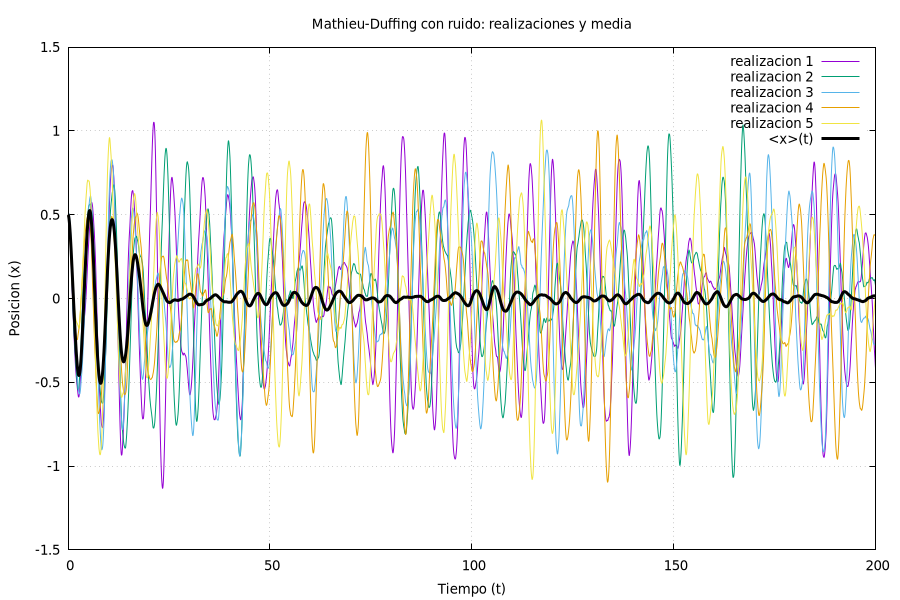
\includegraphics[width=0.78\textwidth]{trayectorias.png}
    \caption{Cinco realizaciones y media del ensamble ($h=0.5$, $\sigma=0.2$, Heun, $N=200$, semilla $12345$).}
    \label{fig:tray}
\end{figure}

\begin{figure}[H]
    \centering
    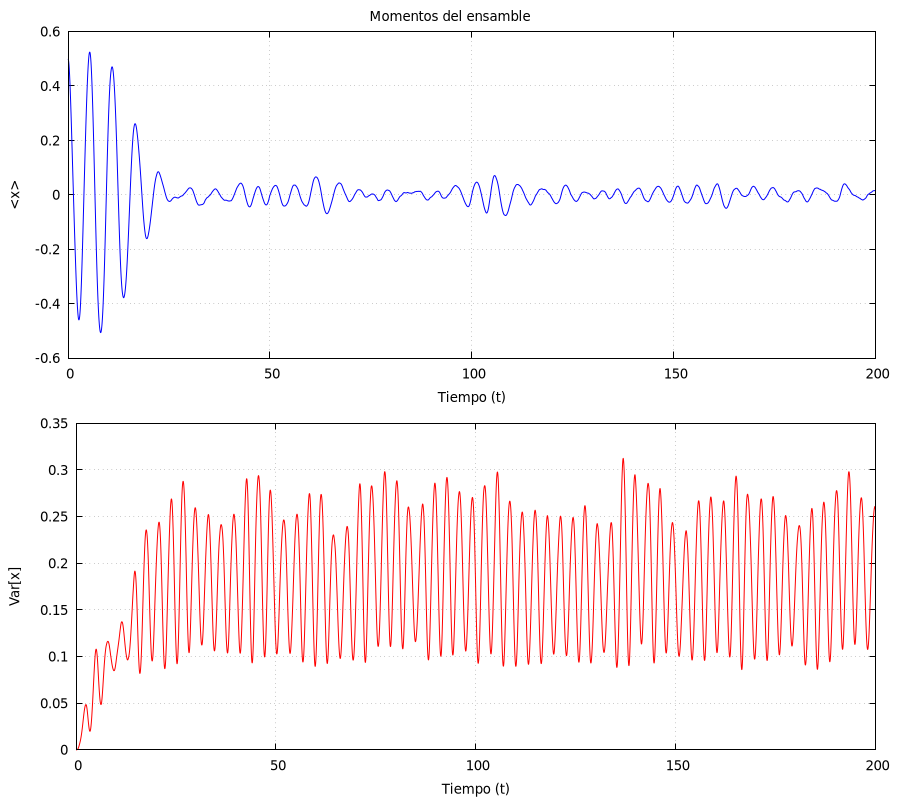
\includegraphics[width=0.66\textwidth]{momentos.png}
    \caption{Media $\media{x}(t)$ y varianza $\mathrm{Var}[x](t)$ del ensamble.}
    \label{fig:mom}
\end{figure}

\begin{figure}[H]
    \centering
    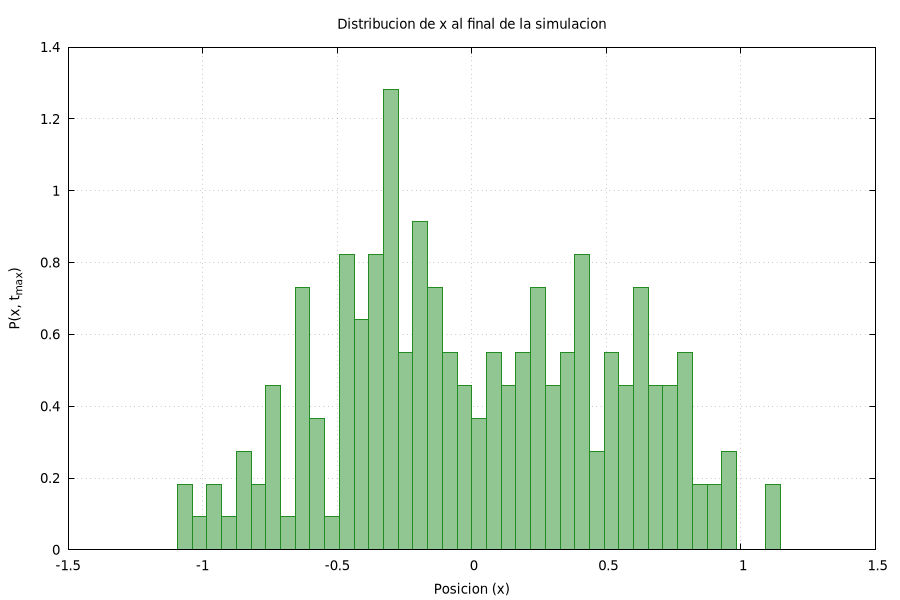
\includegraphics[width=0.66\textwidth]{histograma.png}
    \caption{Histograma normalizado de $x(t_{\max})$ para las $200$ realizaciones.}
    \label{fig:hist}
\end{figure}

\subsection{Validación con el límite lineal}

\begin{table}[H]
\centering
\begin{tabular}{@{}cccccc@{}}
\toprule
$\Delta t$ & Euler-Maruyama & Sesgo [\%] & Heun & Desviación [\%] & Teoría\\
\midrule
$0.2$ & $0.4241$ & $+69.6$ & $0.2467$ & $-1.3$ & $0.25$\\
$0.1$ & $0.3104$ & $+24.2$ & $0.2514$ & $+0.6$ & $0.25$\\
$0.05$ & $0.2818$ & $+12.7$ & $0.2491$ & $-0.4$ & $0.25$\\
$0.025$ & $0.2599$ & $+4.0$ & $0.2444$ & $-2.2$ & $0.25$\\
\bottomrule
\end{tabular}
\caption{$\mathrm{Var}[x(t_{\max})]$ en el límite lineal ($\delta=0.5$, $\sigma=0.5$, $N=20\,000$) y valor exacto $\sigma^{2}/(2\delta\omega_0^{2})=0.25$. El error estadístico es $\sqrt{2/(N-1)}\approx1$~\%.}
\label{tab:lineal}
\end{table}

Euler-Maruyama sobreestima la varianza, y el sesgo disminuye al reducir el paso, aproximadamente en proporción a $\Delta t$ (el error estadístico es del orden del $1$~\%, así que el valor de $4$~\% es poco preciso). Heun reproduce el valor exacto en todos los pasos, con desviaciones de $0.4$ a $2.2$~\%; la mayor, en $\Delta t=0.025$, equivale a unos dos errores estadísticos (Figura~\ref{fig:lineal}).

\begin{figure}[H]
    \centering
    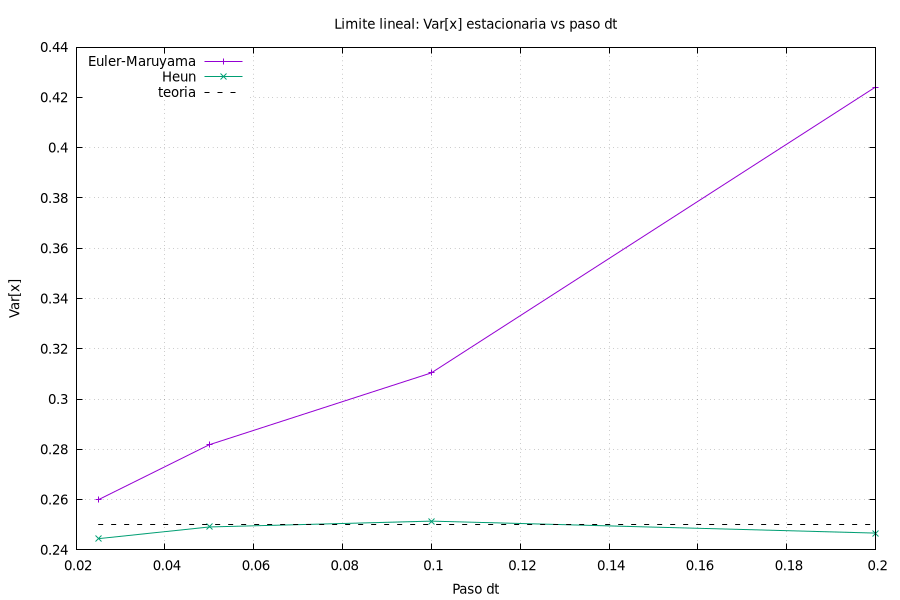
\includegraphics[width=0.78\textwidth]{validacion_lineal.png}
    \caption{Varianza estacionaria frente al paso $\Delta t$ para ambos esquemas; la línea punteada es el valor exacto.}
    \label{fig:lineal}
\end{figure}

\subsection{Convergencia fuerte}

\begin{table}[H]
\centering
\begin{tabular}{@{}cccc@{}}
\toprule
$\Delta t$ & Euler-Maruyama & Heun & Cociente EM/Heun\\
\midrule
$2.44\times10^{-3}$ & $1.26\times10^{-3}$ & $1.79\times10^{-4}$ & $7.1$\\
$4.88\times10^{-3}$ & $2.57\times10^{-3}$ & $4.04\times10^{-4}$ & $6.4$\\
$9.77\times10^{-3}$ & $5.13\times10^{-3}$ & $7.51\times10^{-4}$ & $6.8$\\
$1.95\times10^{-2}$ & $1.02\times10^{-2}$ & $1.63\times10^{-3}$ & $6.3$\\
$3.91\times10^{-2}$ & $2.10\times10^{-2}$ & $3.03\times10^{-3}$ & $6.9$\\
\bottomrule
\end{tabular}
\caption{Error fuerte $\media{|x(T)-x_{\mathrm{ref}}(T)|}$ con $T=5$ ($h=0.5$, $\sigma=0.2$, $300$ caminos).}
\label{tab:fuerte}
\end{table}

El orden calculado con pasos consecutivos es $1.02$, $1.00$, $1.00$ y $1.03$ para Euler-Maruyama, y $1.18$, $0.90$, $1.12$ y $0.90$ para Heun; el ajuste log-log sobre los cinco pasos da pendientes de $1.01$ y $1.02$. Ambos esquemas tienen, por tanto, orden fuerte $\approx1$. Heun no gana en el orden sino en la constante: su error es unas 6 a 7 veces menor (Figura~\ref{fig:fuerte}). La dispersión de los órdenes de Heun refleja el ruido estadístico de promediar solo $300$ caminos.

\begin{figure}[H]
    \centering
    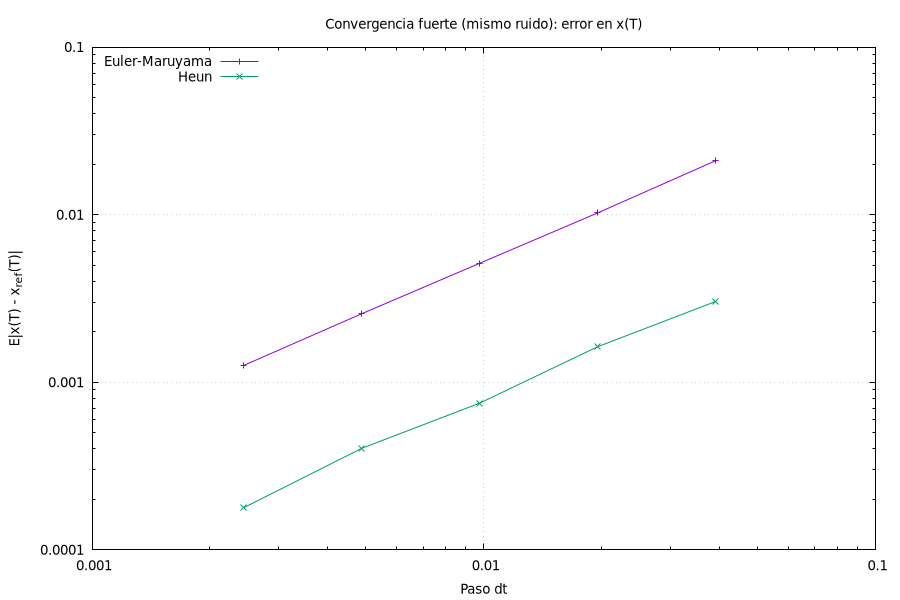
\includegraphics[width=0.78\textwidth]{convergencia_fuerte.png}
    \caption{Error fuerte en $x(T)$ frente al paso $\Delta t$ (escala logarítmica). Las rectas son paralelas, de pendiente $\approx1$.}
    \label{fig:fuerte}
\end{figure}

\subsection{Dependencia con la intensidad del ruido }

\begin{table}[H]
\centering
\begin{tabular}{@{}ccc@{}}
\toprule
$\sigma$ & $\media{x^{2}}$ con $h=0.1$ (bajo el umbral) & $\media{x^{2}}$ con $h=0.5$ (sobre el umbral)\\
\midrule
$0$ & $3\times10^{-6}$ & $0.1519$\\
$0.02$ & $0.0026$ & $0.1498$\\
$0.05$ & $0.0151$ & $0.1362$\\
$0.10$ & $0.0496$ & $0.1257$\\
$0.15$ & $0.0914$ & $0.1510$\\
$0.20$ & $0.1442$ & $0.1869$\\
$0.30$ & $0.2720$ & $0.3038$\\
\bottomrule
\end{tabular}
\caption{Respuesta cuadrática media estacionaria (promedio sobre $N=300$ realizaciones y sobre $t\in(100,200]$).}
\label{tab:sigma}
\end{table}

\paragraph{Por debajo del umbral ($h=0.1$).} Sin ruido, la oscilación decae a cero. Con ruido, $\media{x^{2}}$ crece de forma monótona con $\sigma$, aproximadamente como $\sigma^{2}$. Como referencia, el oscilador lineal sin modulación daría $\sigma^{2}/(2\delta\omega_0^{2})=5\sigma^{2}$ por la ecuación~\eqref{eq:ou}: $0.0125$ para $\sigma=0.05$ y $0.20$ para $\sigma=0.2$, frente a los valores medidos $0.0151$ y $0.1442$. Los valores medidos quedan por encima del lineal a $\sigma$ pequeña y por debajo a $\sigma$ grande; no se separó cuánto aporta la modulación y cuánto el término cúbico.

\paragraph{Por encima del umbral ($h=0.5$).} Sin ruido hay una oscilación sostenida: $\media{x^{2}}=0.1519$ corresponde a una amplitud equivalente de $\sqrt{2\cdot0.1519}\approx0.55$. Con ruido, $\media{x^{2}}$ \emph{no es monótona}: baja hasta $0.1257$ en $\sigma=0.1$ y luego sube, alcanzando $0.1869$ en $\sigma=0.2$ y $0.3038$ en $\sigma=0.3$. A $\sigma=0.2$ el valor coincide con el $\mathrm{Var}[x]\approx0.186$ de la simulación principal (otra semilla, otro $N$ y otra ventana). Con cinco semillas distintas para $\sigma=0.1$ se obtiene $0.1207\pm0.0015$ (desviación estándar entre semillas). El punto del barrido, $0.1257$, queda unos tres desvíos por encima de esa media, de modo que la incertidumbre por semilla de cada punto del barrido es probablemente algo mayor que $0.002$. La caída ($\approx17$~\% respecto al caso sin ruido) es mucho mayor que esa dispersión, pero su causa no se investigó (Figura~\ref{fig:sigma}). A $\sigma=0.3$ las dos curvas casi se juntan: el ruido domina y la diferencia entre estar por debajo o por encima del umbral se pierde.

\begin{figure}[H]
    \centering
    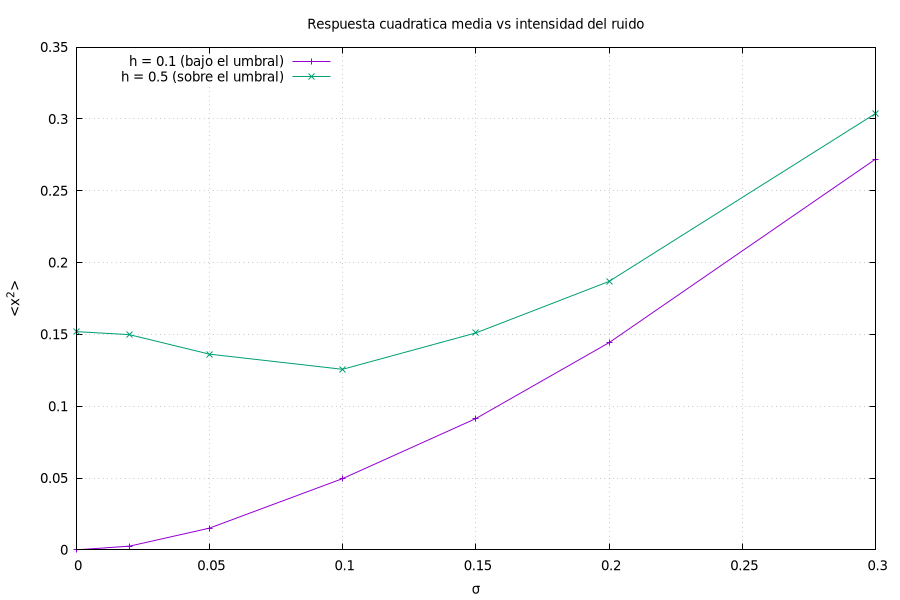
\includegraphics[width=0.78\textwidth]{barrido_sigma.png}
    \caption{$\media{x^{2}}$ estacionario frente a $\sigma$, por debajo ($h=0.1$) y por encima ($h=0.5$) del umbral.}
    \label{fig:sigma}
\end{figure}

\subsection{Mapa estroboscópico}

\begin{table}[H]
\centering
\begin{tabular}{@{}cccc@{}}
\toprule
$\sigma$ & Valores distintos (de $1500$) & Desv.\ est.\ de $x$ & Desv.\ est.\ de $v$\\
\midrule
$0$ & $2$ & $0.110$ & $0.581$\\
$0.05$ & $489$ & $0.132$ & $0.548$\\
$0.2$ & $850$ & $0.311$ & $0.604$\\
\bottomrule
\end{tabular}
\caption{Mapa estroboscópico a $h=0.5$. Los valores distintos se cuentan redondeando a tres decimales.}
\label{tab:estrobo}
\end{table}

Sin ruido hay exactamente dos puntos, $(x,v)=(\mp0.1103,\,\pm0.5805)$, uno el negativo del otro: es la respuesta de período $2T$, con $x(t+T)=-x(t)$. Con $\sigma=0.05$ cada punto se ensancha en una nube compacta alrededor de su posición determinista; con $\sigma=0.2$ las nubes son anchas y se solapan (Figura~\ref{fig:estrobo}).

\begin{figure}[H]
    \centering
    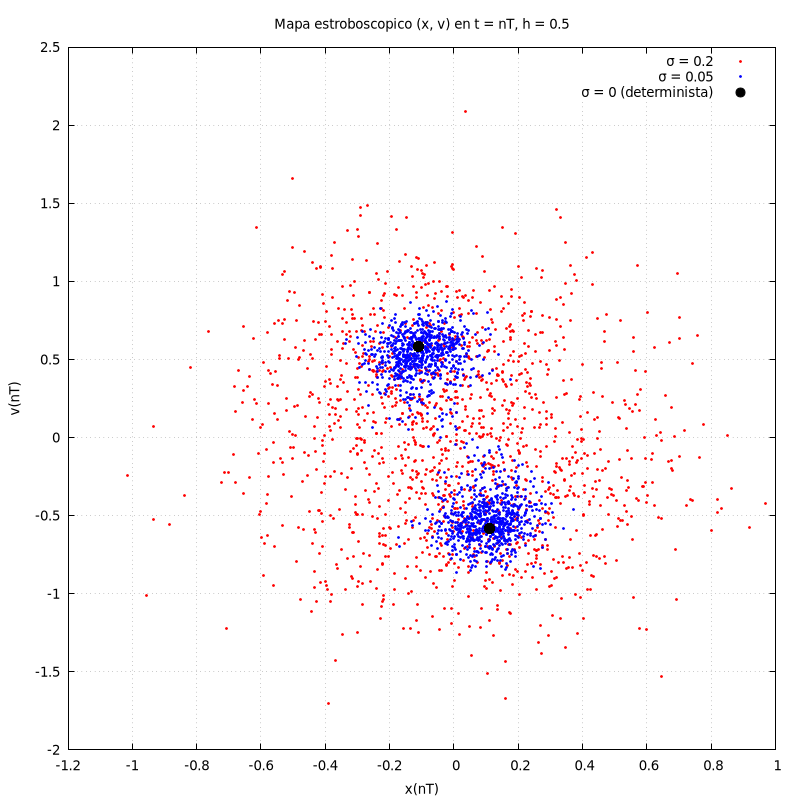
\includegraphics[width=0.62\textwidth]{estroboscopico.png}
    \caption{Mapa estroboscópico $(x,v)$ en $t=nT$ con $h=0.5$: determinista (puntos negros), $\sigma=0.05$ (azul) y $\sigma=0.2$ (rojo).}
    \label{fig:estrobo}
\end{figure}

\subsection{Autocorrelación y espectro}

\begin{table}[H]
\centering
\small
\begin{tabular}{@{}>{\raggedright\arraybackslash}p{5.4cm}>{\centering\arraybackslash}p{4.2cm}>{\centering\arraybackslash}p{4.2cm}@{}}
\toprule
 & $h=0.1$, $\sigma=0.1$ & $h=0.5$, $\sigma=0.05$\\
\midrule
Pico del espectro, $\omega$ & $1.043$ & $0.997$\\
Altura del pico, $S$ & $0.115$ & $2.99$\\
Ancho a media altura (aprox.) & $0.169$ & $0.031$\\
Período de la autocorrelación & $6.21$ & $6.29$\\
$C$ en los primeros máximos ($\tau\approx6,12,18,24$) & $0.72,\ 0.49,\ 0.31,\ 0.17$ & $0.94,\ 0.88,\ 0.86,\ 0.85$\\
$C$ en $\tau\approx50$ & $0.04$ & $0.77$\\
Componente en $\omega\approx3$ & sin pico visible & $S\approx1.6\times10^{-3}$ en $\omega=3.007$\\
\bottomrule
\end{tabular}
\caption{Resultados de autocorrelación y espectro. La resolución en frecuencia es $\Delta\omega=2\pi/(M\Delta t_s)=0.0153$.}
\label{tab:espectro}
\end{table}

Por debajo del umbral, la autocorrelación oscila con período $\approx6.2$ ($\omega\approx1$) y su envolvente cae por debajo de $1/e$ hacia $\tau\approx18$, unos tres ciclos (Figura~\ref{fig:corr}); el espectro tiene un pico ancho y bajo cerca de $\omega=1$ (Figura~\ref{fig:esp}). Por encima del umbral, la autocorrelación casi no decae (de $0.94$ a $0.75$ en $\tau\approx56$), con período $6.29\approx2\pi$, es decir, frecuencia $\Omega/2=1$; el espectro tiene un pico muy estrecho en $\omega=0.997$, unas $26$ veces más alto que el de $h=0.1$, y un pico pequeño en $\omega=3$.

\begin{figure}[H]
    \centering
    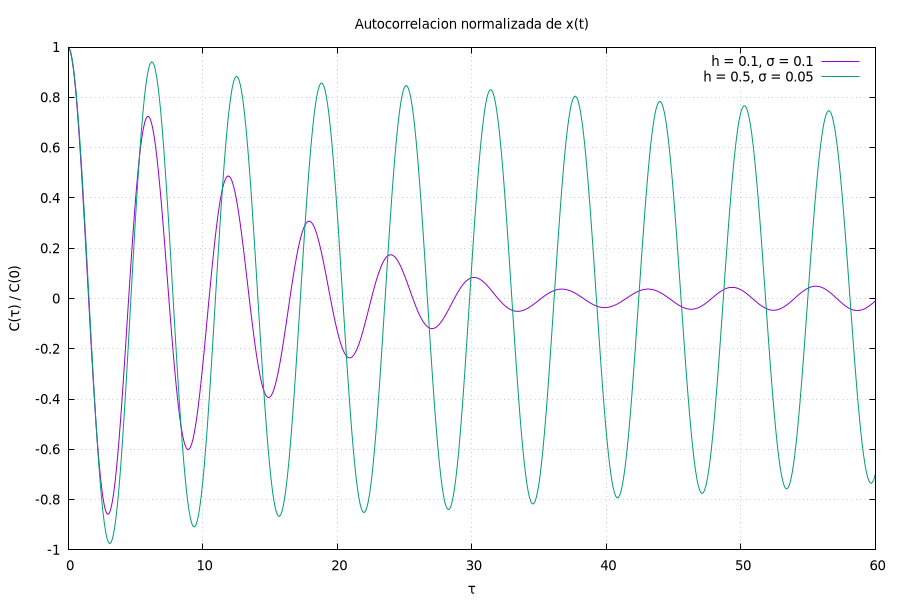
\includegraphics[width=0.78\textwidth]{autocorrelacion.png}
    \caption{Autocorrelación normalizada de $x(t)$ por debajo y por encima del umbral.}
    \label{fig:corr}
\end{figure}

\begin{figure}[H]
    \centering
    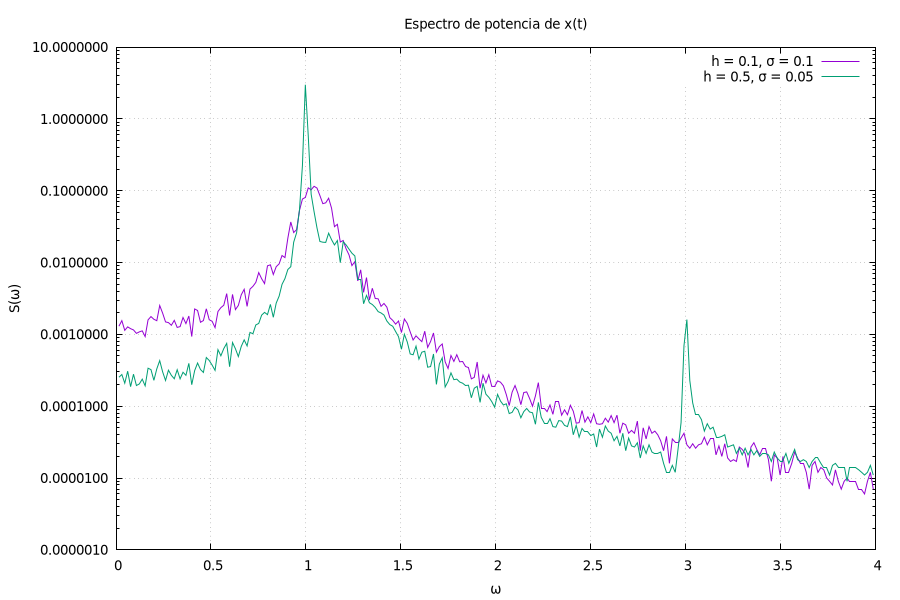
\includegraphics[width=0.78\textwidth]{espectro.png}
    \caption{Espectro de potencia de $x(t)$ (escala logarítmica en $S$), promedio de $20$ realizaciones.}
    \label{fig:esp}
\end{figure}

\section{Conclusiones}

\begin{enumerate}[label=\textbf{\arabic*.}]
    \item El código reproduce el límite lineal exacto: con Heun, $\mathrm{Var}[x]=0.25$ dentro del $\approx2$~\% para todos los pasos probados, mientras que Euler-Maruyama presenta un sesgo de $+4$~\% a $+70$~\% que crece con $\Delta t$.
    \item Con ruido aditivo, Euler-Maruyama y Heun tienen orden fuerte $\approx1$ (observado $1.0$ y $\approx1.0$--$1.2$); Milstein coincide con Euler-Maruyama. Heun tiene un error 6 a 7 veces menor a igual paso y se eligió para las corridas de física.
    \item Para $h=0.5$ y $\sigma=0.2$, el ensamble pierde la media ($\media{x}\approx0$ desde $t\approx20$) y alcanza un régimen en el que $\mathrm{Var}[x]$ oscila con el período del forzamiento, entre $0.086$ y $0.312$, con promedio $0.186$.
    \item Por debajo del umbral ($h=0.1$), $\media{x^{2}}$ crece aproximadamente como $\sigma^{2}$. Por encima ($h=0.5$) parte de $0.152$ sin ruido, disminuye hasta $\approx0.12$--$0.13$ cerca de $\sigma=0.1$ y luego crece; el mecanismo de esa disminución queda sin explicar.
    \item El mapa estroboscópico distingue dinámica y ruido: sin ruido son dos puntos simétricos (período $2T$) y con ruido son nubes alrededor de ellos.
    \item La autocorrelación y el espectro distinguen los dos regímenes: por debajo del umbral hay un pico ancho en $\omega\approx1.04$ y memoria de unos tres ciclos; por encima, un pico estrecho en $\omega\approx\Omega/2$, autocorrelación casi sin decaimiento y un armónico débil en $3\omega$.
    \item Los datos de todos los experimentos se reproducen exactamente con las semillas fijas del código.
\end{enumerate}

\begin{thebibliography}{9}
\bibitem{landau1976} L.~D. Landau y E.~M. Lifshitz, \textit{Mechanics}, 3.ª ed., Butterworth-Heinemann (1976), §27 (resonancia paramétrica).
\bibitem{nayfeh1979} A.~H. Nayfeh y D.~T. Mook, \textit{Nonlinear Oscillations}, Wiley (1979).
\bibitem{kloeden1992} P.~E. Kloeden y E. Platen, \textit{Numerical Solution of Stochastic Differential Equations}, Springer (1992).
\bibitem{higham2001} D.~J. Higham, ``An algorithmic introduction to numerical simulation of stochastic differential equations'', \textit{SIAM Review} \textbf{43}, 525--546 (2001).
\bibitem{gardiner2009} C.~W. Gardiner, \textit{Stochastic Methods: A Handbook for the Natural and Social Sciences}, 4.ª ed., Springer (2009).
\bibitem{matsumoto1998} M. Matsumoto y T. Nishimura, ``Mersenne Twister: a 623-dimensionally equidistributed uniform pseudo-random number generator'', \textit{ACM Transactions on Modeling and Computer Simulation} \textbf{8}, 3--30 (1998).
\end{thebibliography}

\end{document}
